\chapter{الكيمياء العضوية الفلزية: الترابط والربائط}\label{ch:b3:organometallic-bonding}

في سنة 1951 حصلت مجموعتا بحث، كل منهما مستقلة عن الأخرى، على مسحوق برتقالي مستقر
في الهواء صيغته $\ce{FeC10H10}$ لم يكن له معنى: فالحديد لا يكوّن عادة
روابط مستقرة مع الكربون، ولا مع حلقتي سيكلوبنتاديينيل في آن واحد قطعًا.
وفي غضون سنة ثبتت بنيته: فالحديد يجلس بين حلقتين
متوازيتين، مرتبطًا بالتساوي بذرات الكربون العشر كلها، كالشطيرة. وقد
فتح الفيروسين باب الكيمياء العضوية الفلزية الحديثة، التي تصنع حفازاتها اليوم معظم
بوليمرات العالم وأدويته ومواده الكيميائية الدقيقة (\cref{ch:b3:homogeneous-catalysis}).
ويفسّر هذا الفصل كيف ترتبط الفلزات بأحادي أكسيد الكربون والفوسفينات والألكينات
والحلقات والكربينات وبعضها ببعض، وكيف يصل \omterm{def:b3:organometallic-bonding:isolobal}{التماثل المتساوي الفصوص}
الشظايا العضوية الفلزية بالكيمياء العضوية للكربون.

\begin{recall}
عرّف مجلد السنة الأولى المركبات العضوية الفلزية واستعمل كواشف غرينيار.
وقدّم مجلد السنة الثانية قاعدة الثمانية عشر إلكترونًا وعدّ إلكترونات التكافؤ، 
والهابتية، والربائط المستقبلة $\pi$ والمانحة $\pi$ مع التبرع العكسي، والخطوات
الأولية للتفاعلات العضوية الفلزية (الإضافة التأكسدية، والحذف الاختزالي،
والإدخال) ومدارات الشظايا. وعدّ \cref{ch:b3:group-theory-applied}
اهتزازات تمدد CO النشطة في تحت الأحمر في الكربونيلات وبنى التراكيب
المتكيفة مع التناظر؛ وربط \cref{ch:b3:complex-spectra-magnetism} العزوم المغناطيسية
بالإلكترونات المنفردة.
\end{recall}

\begin{omfigure}
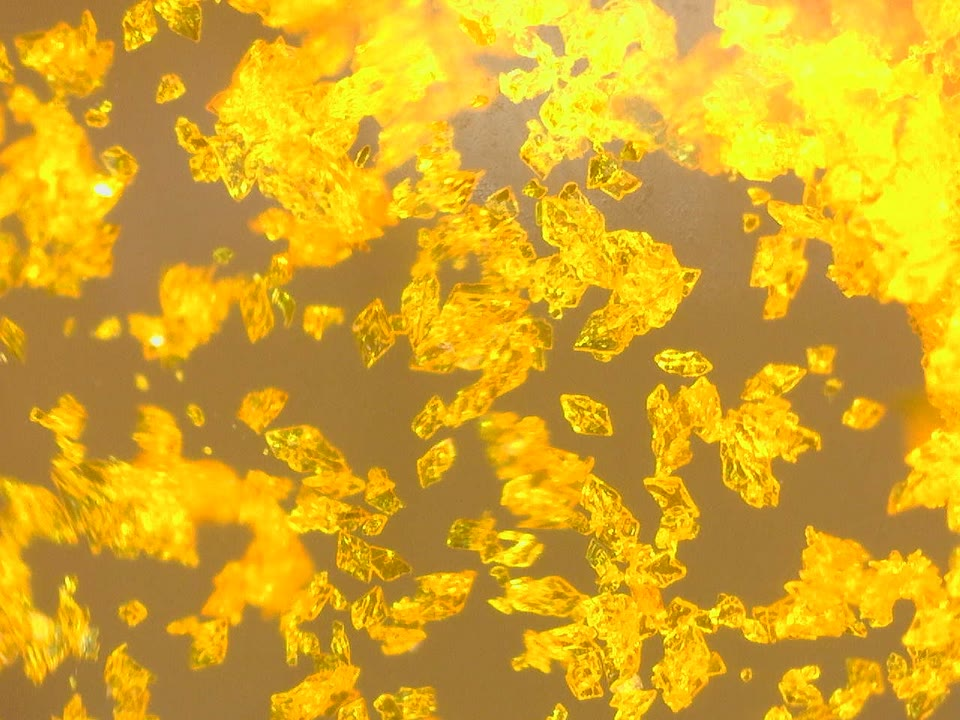
\includegraphics[width=0.5\linewidth]{images/book4/ferrocene-crystals.jpg}

{\small بلورات الفيروسين، $\ce{Fe(C5H5)2}$: مركب عضوي فلزي برتقالي
مستقر في الهواء، يتسامى بالتسخين اللطيف.}
\end{omfigure}

\section{عدّ الإلكترونات وحالات الأكسدة}

\begin{method}[عدّ الإلكترونات بطريقتين]\label{met:b3:organometallic-bonding:count}
\begin{enumerate}
  \item طريقة الربائط المتعادلة (التساهمية): يقدّم الفلز عددًا من الإلكترونات يساوي رقم
        مجموعته؛ وكل ربيطة، مأخوذةً متعادلة، تقدّم 1 (H، \ce{CH3}، Cl،
        الأليل $\eta^1$) أو 2 (CO، \ce{PR3}، ألكين) أو أكثر ($\eta^5$-\ce{C5H5} 5، $\eta^6$-\ce{C6H6} 6)؛ وأضف واحدًا لكل
        رابطة فلز--فلز وصحّح بحسب الشحنة الإجمالية.
  \item الطريقة الأيونية: تُعدّ الربائط مثل H و\ce{CH3} وCl و\ce{C5H5} أنيونات (2 و2
        و2 و6 إلكترونات)، ويُعدّ الفلز الكاتيونَ $d^n$ الناتج؛ والربائط المتعادلة
        كما سبق.
  \item تعطي الطريقتان المجموع نفسه؛ وتعطي الطريقة الأيونية أيضًا حالة الأكسدة
        وعدد $d^n$.
\end{enumerate}
\end{method}

\begin{example}[العدّ]\label{ex:b3:organometallic-bonding:count}
$\ce{Fe(CO)5}$: $8 + 5 \times 2 = 18$، حديد(0)، $d^8$. الفيروسين: الطريقة المتعادلة $8 + 2 \times 5 = 18$؛ والطريقة الأيونية
$\ce{Fe^{2+}}$ ($d^6$، 6) $+ 2 \times 6$ ($\ce{C5H5-}$) $= 18$، حديد(II). $\ce{Mn2(CO)10}$: كل Mn $7 + 5 \times 2 + 1$ (الرابطة Mn--Mn)
$= 18$. والمعقدات المربعة المستوية $d^8$ مثل $\ce{[PtCl4]^{2-}}$ أو حفاز ويلكنسون
$\ce{RhCl(PPh3)3}$ لها 16 إلكترونًا: فمدارها الفارغ الشبيه بالمدار $p_z$ أعلى من أن يُملأ، 
والمعقدات المربعة المستوية ذات الستة عشر إلكترونًا مستقرة استقرار المعقدات ذات الثمانية عشر إلكترونًا.
\end{example}

\section{الكربونيلات والفوسفينات}

\begin{definition}[الكربونيلات الفلزية]\label{def:b3:organometallic-bonding:carbonyl}
\emph{الكربونيل الفلزي}\index{كربونيل فلزي} معقد ربائطه من أحادي أكسيد
الكربون. و\emph{الكربونيل الطرفي}\index{كربونيل طرفي} يرتبط بفلز
واحد عبر الكربون؛ و\emph{الكربونيل الجسري}\index{كربونيل جسري} يمتد
بين فلزين (أو ثلاثة).
\end{definition}

وجد لودفيغ موند في سنة 1890 أن النيكل يتفاعل مع أحادي أكسيد الكربون عند درجة
الحرارة العادية فيعطي السائل المتطاير $\ce{Ni(CO)4}$، الذي يتفكك عائدًا إلى نيكل
نقي بالتسخين: وهذا أساس طريقة لتنقيته. ويرتبط أحادي أكسيد الكربون
بالفلزات الانتقالية عبر أعلى مداراته المشغولة، وهو زوج حر $\sigma$ متمركز معظمه
على الكربون، ويستقبل إلكترونات في مداريه الفارغين $\pi^*$، الأكبر أيضًا على
الكربون.

\begin{definition}[الارتباط التآزري]\label{def:b3:organometallic-bonding:synergic}
\emph{الارتباط التآزري}\index{ارتباط تآزري} هو التعزيز المتبادل بين
التبرع $\sigma$ من ربيطة إلى فلز والتبرع العكسي $\pi$ من الفلز إلى
الربيطة: فالتبرع يجعل الفلز أغنى بالإلكترونات وأكثر استعدادًا لإعادتها،
والتبرع العكسي يخفف الشحنة التي تراكمت بالتبرع.
\end{definition}

\begin{omfigure}
\begin{tikzpicture}[font=\small, >=Stealth]
  % sigma donation
  \fill[black!70] (0,0) circle (0.14); \node[anchor=north] at (0,-0.4) {M};
  \pic at (0,0) {omlobe={-0.7}{180}};
  \pic at (0,0) {omlobe={0.9}{0}};
  \node[circle, fill=black!40, inner sep=1.6pt] at (1.9,0) {};
  \node[circle, fill=omThm!70, inner sep=1.6pt] at (3.0,0) {};
  \pic at (1.9,0) {omlobe={0.85}{180}};
  \node[font=\scriptsize, anchor=north] at (1.9,-0.25) {C};
  \node[font=\scriptsize, anchor=north] at (3.0,-0.25) {O};
  \draw[->, thick, omThm] (1.4,0.55) to[bend right=30] (0.6,0.55);
  \node[anchor=north] at (1.5,-1.55) {\foreignlanguage{arabic}{تبرع $\sigma$}};
  % pi back-donation
  \begin{scope}[xshift=6.0cm]
    \fill[black!70] (0,0) circle (0.14); \node[anchor=north] at (0,-1.1) {M};
    \pic at (0,0) {omdxz};
    \node[circle, fill=black!40, inner sep=1.6pt] at (1.9,0) {};
    \node[circle, fill=omThm!70, inner sep=1.6pt] at (3.0,0) {};
    \pic at (1.9,0) {omp={0.9}{90}};
    \pic at (3.0,0) {omp={-0.6}{90}};
    \draw[->, thick, omThm] (0.6,1.05) to[bend left=30] (1.6,1.05);
    \node[anchor=north] at (1.5,-1.55) {\foreignlanguage{arabic}{تبرع عكسي $\pi$}};
  \end{scope}
\end{tikzpicture}

{\small \omterm{def:b3:organometallic-bonding:synergic}{الارتباط التآزري} لأحادي أكسيد الكربون. يسارًا: الزوج الحر للكربون (المدار $\sigma$)
يتبرع في مدار فلزي فارغ من نمط $\sigma$. يمينًا: مدار $d$ فلزي ممتلئ
($d_{xz}$، بمحوريه) يتداخل مع المدار الفارغ $\pi^*$ للجزيء CO، الأكبر على
الكربون، الذي تتوافق فصوصه مع أطواره: فتعود الإلكترونات إلى مدار
مضاد للترابط بين C وO.}
\end{omfigure}

\begin{proposition}[ترددات تمدد CO]\label{prop:b3:organometallic-bonding:co-frequency}
كلما ازداد التبرع العكسي للفلز في المدارات $\pi^*$ لربيطة CO، انخفض
العدد الموجي لتمدد C--O.
\end{proposition}

\begin{proof}[تعليل]
المداران $\pi^*$ للجزيء CO مضادان للترابط بين C وO: فإشغالهما يُضعف
الرابطة C--O، ويخفض ثابت قوتها، ومنه العدد الموجي للتمدد، الذي
يتغير كالجذر التربيعي \omterm{def:b3:quantum-model-systems:oscillator}{لثابت القوة} (\cref{ch:b3:rovibrational-spectroscopy}).
والتبرع $\sigma$ ينزع إلكترونات من مدار شبه غير رابط (مضاد للترابط قليلًا)
بالنسبة إلى C--O، وهذا وحده يرفع العدد الموجي قليلًا: 
والانخفاض المرصود يبيّن أن التبرع العكسي هو الغالب.
\end{proof}

لأحادي أكسيد الكربون الحر انتقاله الأساسي عند $\omega_e - 2\omega_ex_e = \qty{2143}{cm^{-1}}$؛ 
والكربونيلات الطرفية في المعقدات المتعادلة تمتص تقريبًا بين 1900 و\qty{2100}{cm^{-1}}،
والكربونيلات الجسرية أدنى من ذلك. وعلى امتداد سلسلة متساوية الإلكترونات، يمتص الكربونيل
الأنيوني عند عدد موجي أدنى من المتعادل، والكاتيوني عند
عدد أعلى: فكلما كان الفلز أغنى بالإلكترونات، ازداد تبرعه العكسي. وعدد
الحزم، بحسب التناظر (\cref{ch:b3:group-theory-applied})، يعطي الهندسة.
% ledger: diat:CO.we, diat:CO.wexe

\begin{proposition}[التآثرات $\pi$ وانشطار مجال الربائط]\label{prop:b3:organometallic-bonding:pi-delta}
في معقد ثماني الأوجه، تزيد الربائط المستقبلة $\pi$ قيمة $\Delta_{\mathrm o}$ وتخفضها الربائط
المانحة $\pi$.
\end{proposition}

\begin{proof}
للمدارات $e_g$ تناظر $\sigma$ فقط. أما المدارات $t_{2g}$ ($d_{xy}$، $d_{xz}$، $d_{yz}$) فتوافق تركيبًا $t_{2g}$
لمدارات $\pi$ للربائط: فمن أجل $d_{xy}$، تقدّم كل ربيطة من الربائط الأربع الواقعة في المستوي $xy$
مدارًا $\pi$ عموديًا على محورها M--L في ذلك المستوي، 
والتركيب ذو الإشارات المتناوبة له تناظر $d_{xy}$ (والتراكيب
الباقية تتحول وفق $t_{1g}$ و$t_{1u}$ و$t_{2u}$ ولا تجد شريكًا $d$). والمداران
المتماثلا التناظر يمتزجان ويتنافران: فيُدفع الأدنى إلى الأسفل والأعلى إلى الأعلى. 
والمستقبل $\pi$ يقدّم مدارات فارغة فوق المجموعة $t_{2g}$، فتُدفع هذه إلى الأسفل: فتزداد $\Delta_{\mathrm o}$.
والمانح $\pi$ يقدّم مدارات ممتلئة تحتها، تدفعها إلى الأعلى: فتنقص $\Delta_{\mathrm o}$.
ولا يتأثر المستوى $e_g$ في الحالتين.
\end{proof}

لهذا يقع CO و\ce{CN-} في الطرف القوي من السلسلة الطيفية الكيميائية، 
والهاليدات والهيدروكسيد في الطرف الضعيف، كما ذكر مجلد السنة الثانية.

\begin{definition}[وسيطا تولمان]\label{def:b3:organometallic-bonding:tolman}
\emph{زاوية مخروط تولمان}\index{زاوية مخروط تولمان} لفوسفين هي زاوية
رأس المخروط، المتمركز على الفلز عند مسافة معيارية، الذي يحيط بالكاد
بسطوح فان دير فالس لمستبدلاته: وهي مقياس لحجمه.
و\emph{الوسيط الإلكتروني لتولمان}\index{وسيط تولمان الإلكتروني} هو
العدد الموجي لتمدد CO المتناظر في $\ce{Ni(CO)3L}$: فكلما كان تبرع
الفوسفين L أقوى، كان أدنى.
\end{definition}

تُضبط الفوسفينات حجمًا وتبرعًا إلكترونيًا كلًّا على حدة بواسطة
مستبدلاتها: فثلاثيات ألكيل الفوسفين مانحات أقوى من ثلاثيات أريل الفوسفين،
والفوسفيتات أضعفها؛ و$\ce{P(tBu)3}$ أضخم بكثير من $\ce{PMe3}$. والفوسفينات الضخمة تفضّل
أعداد التناسق المنخفضة وتفكك الربائط السريع، ولهذا
تظهر في حفازات كثيرة جدًا.

\section{الربائط $\pi$}

\begin{definition}[نموذج ديوار--تشات--دنكانسون]\label{def:b3:organometallic-bonding:dcd}
\emph{نموذج ديوار--تشات--دنكانسون}\index{نموذج ديوار--تشات--دنكانسون} لارتباط
ألكين بفلز يجمع بين التبرع $\sigma$ من المدار $\pi$ للرابطة C=C
إلى مدار فلزي فارغ والتبرع العكسي من مدار $d$ فلزي ممتلئ إلى
المدار $\pi^*$ للرابطة C=C. وحدّه عند تبرع عكسي قوي هو
\emph{حلقي البروبان الفلزي}\index{حلقي بروبان فلزي}، أي حلقة ثلاثية
فيها رابطتان $\sigma$ من نوع M--C ورابطة أحادية C--C.
\end{definition}

\begin{proposition}[عواقب التبرع العكسي إلى ألكين]\label{prop:b3:organometallic-bonding:dcd}
يطيل التناسق الرابطة C=C ويثني المستبدلات إلى الخلف، بعيدًا عن
الفلز، وأكثر كلما ازداد التبرع العكسي.
\end{proposition}

\begin{proof}[تعليل]
نزع إلكترونات من المدار $\pi$ (الرابط) وإضافتها إلى المدار $\pi^*$
(المضاد للترابط) كلاهما يخفض رتبة الرابطة C--C. ومزج الطابع $\pi^*$
يعيد تهجين ذرتي الكربون نحو $sp^3$، التي تتجه روابطها بالمستبدلات بعيدًا
عن الفلز، نحو هندسة \omterm{def:b3:organometallic-bonding:dcd}{حلقي البروبان الفلزي}.
\end{proof}

\begin{omfigure}
\begin{tikzpicture}[font=\small, >=Stealth]
  \fill[black!70] (0,0) circle (0.14); \node[anchor=north] at (0,-1.1) {M};
  \pic at (0,0) {omlobe={0.9}{0}};
  \foreach \y in {0.45,-0.45}{\node[circle, fill=black!40, inner sep=1.6pt] at (1.9,\y) {};}
  \pic at (1.9,0.45) {omp={-0.75}{0}};
  \pic at (1.9,-0.45) {omp={-0.75}{0}};
  \draw[->, thick, omThm] (1.3,1.0) to[bend right=30] (0.5,0.6);
  \node[anchor=north] at (1.2,-1.4) {$\sigma$: $\pi$(C=C) $\to$ M};
  \begin{scope}[xshift=5.6cm]
    \fill[black!70] (0,0) circle (0.14); \node[anchor=north] at (0,-1.1) {M};
    \pic at (0,0) {omdxy};
    \foreach \y in {0.45,-0.45}{\node[circle, fill=black!40, inner sep=1.6pt] at (1.9,\y) {};}
    \pic at (1.9,0.45) {omp={-0.75}{0}};
    \pic at (1.9,-0.45) {omp={0.75}{0}};
    \draw[->, thick, omThm] (0.7,0.9) to[bend left=30] (1.5,0.9);
    \node[anchor=north] at (1.2,-1.4) {$\pi$: M $\to$ $\pi^*$(C=C)};
  \end{scope}
\end{tikzpicture}

{\small \omterm{def:b3:organometallic-bonding:dcd}{نموذج ديوار--تشات--دنكانسون} لألكين مرتبط جانبيًا (الرابطة C=C
عمودية، والفلز على اليسار). يسارًا: المدار $\pi$ الممتلئ (مداران $p$ متوافقا
الطور) يتبرع في مدار فلزي فارغ. يمينًا: مدار $d$ فلزي ممتلئ
متوافق الأطوار يتبرع في المدار الفارغ $\pi^*$ (المداران $p$ متعاكسا
الطور).}
\end{omfigure}

ملح زايزه، $\ce{K[PtCl3(C2H4)]}$، المحضَّر سنة 1827، كان أول مركب عضوي فلزي
لفلز انتقالي؛ وجزيء الإيثين فيه عمودي على المستوي \ce{PtCl3}، كما
يتنبأ النموذج. والأليل ($\eta^3$) والديينات ($\eta^4$) والأرينات ($\eta^6$) وحلقة
السيكلوبنتاديينيل ($\eta^5$) ترتبط بالطريقة نفسها عبر عدة ذرات كربون في آن واحد.

\begin{definition}[الميتالوسينات]\label{def:b3:organometallic-bonding:metallocene}
\emph{المركب الشطيري}\index{مركب شطيري} فيه فلز بين ربيطتين حلقيتين
مستويتين متوازيتين مرتبطتين عبر كل ذرات كربونهما؛ 
و\emph{الميتالوسين}\index{ميتالوسين} مركب شطيري فيه حلقتا سيكلوبنتاديينيل $\eta^5$،
$\ce{M(C5H5)2}$.
\end{definition}

\begin{proposition}[المدارات الحدودية للفيروسين]\label{prop:b3:organometallic-bonding:ferrocene}
في \omterm{def:b3:organometallic-bonding:metallocene}{ميتالوسين} حلقتاه متوازيتان ($D_{5d}$)، تنشطر المدارات $d$ للفلز إلى $e_{2g}$
($d_{xy}$، $d_{x^2-y^2}$) و$a_{1g}$ ($d_{z^2}$)، شبه غير رابطة ومتقاربة، و$e_{1g}^\ast$ ($d_{xz}$،
$d_{yz}$)، مضادة للترابط بشدة؛ وللفيروسين، بإلكتروناته الستة $d$ في $e_{2g}^4a_{1g}^2$، 18
إلكترونًا ولا إلكترون منفرد فيه.
\end{proposition}

\begin{proof}[تعليل]
تتركب المدارات $\pi$ للحلقتين في أزواج متكيفة مع التناظر $a_{1g}$ و$a_{2u}$ 
و$e_{1g}$ و$e_{1u}$ و$e_{2g}$ و$e_{2u}$ (من المدارات $\pi$ الخمسة لكل حلقة، بصفر وواحد واثنين
من المستويات العقدية المارة بالمحور). والتركيب $e_{1g}$ الممتلئ للحلقتين يتداخل
بقوة مع $d_{xz}$ و$d_{yz}$ (لكل منهما مستوٍ عقدي واحد يمر بالمحور): فيكوّنان مدارات رابطة،
معظمها حلقي، ومدارات $e_{1g}^\ast$ مضادة للترابط، معظمها فلزي، مدفوعة إلى الأعلى. أما $d_{xy}$ و$d_{x^2-y^2}$
(بمستويين عقديين) فلا يلاقيان إلا مدارات $e_{2g}$ الفارغة للحلقتين ويستقران قليلًا
بالتبرع العكسي؛ و$d_{z^2}$ يتجه نحو الفجوة في وسط كل حلقة 
ويكاد لا يتداخل. وتملأ ستة إلكترونات $e_{2g}$ و$a_{1g}$؛ ومع الإلكترونات الاثني عشر في
تراكيب الحلقتين الرابطة، يصير العدد 18.
\end{proof}

\begin{omfigure}
\begin{tikzpicture}[font=\small]
  % sandwich drawing
  \begin{scope}[xshift=-1.0cm]
    \draw[thick, fill=black!8] (0,1.0) ellipse (1.0 and 0.3);
    \draw[thick, fill=black!8] (0,-1.0) ellipse (1.0 and 0.3);
    \foreach \a in {90,162,234,306,18}{\fill[black!60] ({cos(\a)},{1.0+0.3*sin(\a)}) circle (0.07);
      \fill[black!60] ({cos(\a)},{-1.0+0.3*sin(\a)}) circle (0.07);}
    \shade[ball color=orange!70!brown] (0,0) circle (0.2);
    \node[anchor=west] at (0.25,0) {Fe};
  \end{scope}
  % level diagram for four metallocenes
  \pic[transform shape] at (2.1,-0.9) {omlevel={u}{0.5}};
  \pic[transform shape] at (2.7,-0.9) {omlevel={ud}{0.5}};
  \pic[transform shape] at (2.4,-0.4) {omlevel={ud}{0.5}};
  \pic[transform shape] at (2.1,1.0) {omlevel={}{0.5}};
  \pic[transform shape] at (2.7,1.0) {omlevel={}{0.5}};
  \node[anchor=north] at (2.4,-1.3) {\ce{[FeCp2]+}};
  \node[anchor=north, font=\scriptsize] at (2.4,-1.75) {17 e$^-$};
  \pic[transform shape] at (4.3,-0.9) {omlevel={ud}{0.5}};
  \pic[transform shape] at (4.9,-0.9) {omlevel={ud}{0.5}};
  \pic[transform shape] at (4.6,-0.4) {omlevel={ud}{0.5}};
  \pic[transform shape] at (4.3,1.0) {omlevel={}{0.5}};
  \pic[transform shape] at (4.9,1.0) {omlevel={}{0.5}};
  \node[anchor=north] at (4.6,-1.3) {\ce{FeCp2}};
  \node[anchor=north, font=\scriptsize] at (4.6,-1.75) {18 e$^-$};
  \pic[transform shape] at (6.5,-0.9) {omlevel={ud}{0.5}};
  \pic[transform shape] at (7.1,-0.9) {omlevel={ud}{0.5}};
  \pic[transform shape] at (6.8,-0.4) {omlevel={ud}{0.5}};
  \pic[transform shape] at (6.5,1.0) {omlevel={u}{0.5}};
  \pic[transform shape] at (7.1,1.0) {omlevel={}{0.5}};
  \node[anchor=north] at (6.8,-1.3) {\ce{CoCp2}};
  \node[anchor=north, font=\scriptsize] at (6.8,-1.75) {19 e$^-$};
  \pic[transform shape] at (8.7,-0.9) {omlevel={ud}{0.5}};
  \pic[transform shape] at (9.3,-0.9) {omlevel={ud}{0.5}};
  \pic[transform shape] at (9.0,-0.4) {omlevel={ud}{0.5}};
  \pic[transform shape] at (8.7,1.0) {omlevel={u}{0.5}};
  \pic[transform shape] at (9.3,1.0) {omlevel={u}{0.5}};
  \node[anchor=north] at (9.0,-1.3) {\ce{NiCp2}};
  \node[anchor=north, font=\scriptsize] at (9.0,-1.75) {20 e$^-$};
  \node[anchor=east, font=\scriptsize] at (1.8,-0.9) {$e_{2g}$};
  \node[anchor=east, font=\scriptsize] at (1.8,-0.4) {$a_{1g}$};
  \node[anchor=east, font=\scriptsize] at (1.8,1.0) {$e_{1g}^\ast$};
\end{tikzpicture}

{\small يسارًا: البنية الشطيرية للفيروسين (حلقتان متطابقتان). يمينًا:
المدارات الحدودية ذات الطابع $d$ في \omterm{def:b3:organometallic-bonding:metallocene}{الميتالوسينات}، $e_{2g}$ و$a_{1g}$ شبه غير رابطة، و$e_{1g}^\ast$
مضادة للترابط، مملوءة من أجل كاتيون الفيروسينيوم (17 إلكترونًا)، والفيروسين (18)،
والكوبالتوسين (19) والنيكلوسين (20، إلكترون واحد في كل مدار $e_{1g}^\ast$، وسبيناهما
متوازيان بحسب قاعدة هوند).}
\end{omfigure}

\section{الكربينات والكرباينات والروابط فلز--فلز}

\begin{definition}[الكربينات ومعقدات الكربين]\label{def:b3:organometallic-bonding:carbene}
\emph{الكربين}\index{كربين} نوع متعادل $\ce{R2C}$ فيه كربون ثنائي التكافؤ
يحمل إلكترونين غير رابطين. و\emph{معقد الكربين}\index{معقد كربين}
فيه ربيطة $\ce{CR2}$ مرتبطة بفلز برابطة مضاعفة، $\ce{M=CR2}$. 
ومعقد \emph{كربين فيشر}\index{كربين فيشر} فيه مستبدل ذرة غير متجانسة
على كربون الكربين وفلز منخفض التكافؤ مع ربائط مستقبلة $\pi$؛ وكربون الكربين فيه
محب للإلكترونات. ومعقد \emph{كربين شروك}\index{كربين شروك} (ألكيليدين)
ليس فيه إلا مستبدلات C أو H وفلز مبكر عالي التكافؤ؛ وكربونه
محب للنواة. و\emph{الكربين الحلقي غير المتجانس النيتروجيني}\index{كربين حلقي غير متجانس نيتروجيني}
كربين حلقي تحيط به ذرتا نيتروجين، مستقر بوصفه مركبًا حرًا، وهو ربيطة
مانحة $\sigma$ قوية.
\end{definition}

يختلف نوعا معقدات \omterm{def:b3:organometallic-bonding:carbene}{الكربين} في طريقة تقاسم الرابطة M=C.
ففي \omterm{def:b3:organometallic-bonding:carbene}{كربين فيشر} يتبرع \omterm{def:b3:organometallic-bonding:carbene}{كربين} أحادي بزوجه الحر للفلز 
ويتلقى تبرعًا عكسيًا في مداره $p$ الفارغ، الذي يثبّته أيضًا الزوج الحر للذرة غير
المتجانسة: فيبقى الكربون فقيرًا بالإلكترونات، تهاجمه المحبات للنواة. وفي
\omterm{def:b3:organometallic-bonding:carbene}{كربين شروك} تكوّن شظيتان ثلاثيتان، الفلز \omterm{def:b3:organometallic-bonding:carbene}{والكربين}، رابطة تساهمية $\sigma +
\pi$، مستقطبة نحو الكربون: فيسلك الألكيليدين سلوك يليد فيتيغ.

\begin{definition}[معقد الكرباين]\label{def:b3:organometallic-bonding:carbyne}
\emph{معقد الكرباين}\index{معقد كرباين} فيه رابطة ثلاثية بين فلز
وكربون يحمل مستبدلًا واحدًا، $\ce{M#CR}$.
\end{definition}

\begin{definition}[الرابطة $\delta$، الرابطة الرباعية]\label{def:b3:organometallic-bonding:delta}
\emph{الرابطة $\delta$}\index{رابطة دلتا@رابطة $\delta$} رابطة لمدارها مستويان عقديان
يحويان المحور بين النوويين، تتكوّن بتداخل مدارين $d$ وجهًا لوجه
مثل $d_{xy}$ و$d_{xy}$. و\emph{الرابطة الرباعية}\index{رابطة رباعية}
تجمع رابطة $\sigma$ ورابطتين $\pi$ ورابطة $\delta$ بين ذرتي فلز.
\end{definition}

\begin{proposition}[{\omterm{def:b3:organometallic-bonding:delta}{الرابطة الرباعية} في $[\mathrm{Re_2Cl_8}]^{2-}$}]\label{prop:b3:organometallic-bonding:quadruple}
في $\ce{[Re2Cl8]^{2-}}$ (ذرتا \ce{Re^{III}}، $d^4$ لكل منهما)، تشغل الإلكترونات $d$ الثمانية $\sigma^2\pi^4\delta^2$: أي رتبة
رابطة 4، وهذا يقتضي الترتيب المتطابق لوحدتي \ce{ReCl4}.
\end{proposition}

\begin{proof}
مع $z$ على امتداد المحور Re--Re وذرات Cl على امتداد $\pm x$ و$\pm y$ عند كل Re، يتجه $d_{x^2-y^2}$
نحو الكلوريدات ويُستعمل في الترابط Re--Cl. أما المدارات $d$ الأربعة الأخرى
لكل فلز فتتداخل مثنى مثنى: $d_{z^2}$ مع $d_{z^2}$ على امتداد المحور ($\sigma$)، و$d_{xz}$ مع $d_{xz}$ و$d_{yz}$
مع $d_{yz}$ جنبًا إلى جنب ($\pi$، مرتين)، و$d_{xy}$ مع $d_{xy}$ وجهًا لوجه ($\delta$، الأضعف).
وتملأ ثمانية إلكترونات التراكيب الرابطة الأربعة. وتدوير إحدى الوحدتين بزاوية $45^\circ$
حول $z$ يحوّل $d_{xy}$ فيها إلى $d_{x^2-y^2}$، الذي يكون تداخله مع $d_{xy}$ الآخر معدومًا بحكم
التناظر: فتضيع الرابطة $\delta$، ومعها تفضيل الترتيب المتطابق. أما
التداخلات الثلاثة الأخرى فمتناظرة أسطوانيًا أو لا يتغير مقدارها.
\end{proof}

% ledger: geom:Re2Cl8.ReRe
المسافة Re--Re البالغة \qty{2.24}{\angstrom} في ملح البوتاسيوم قصيرة جدًا بالنسبة إلى ذرتي فلز، وكلوريدات النصفين متطابقة فعلًا، رغم
تنافرها الفراغي: فالرابطة $\delta$، على ضعفها، هي التي تبقيها كذلك.

\begin{omfigure}
\tdplotsetmaincoords{58}{25}
\begin{tikzpicture}[tdplot_main_coords, font=\small, scale=1.15]
  \draw[thick, black!60] (0,0,0) -- (0,0,2.0);
  \foreach \z in {0,2.0}{
    \foreach \b in {0,90,180,270}{
      \draw[black!45] (0,0,\z) -- ({1.55*cos(\b)},{1.55*sin(\b)},\z);}
    \foreach \a/\s in {45/omphasepos, 135/omphaseneg, 225/omphasepos, 315/omphaseneg}{
      \path[\s, opacity=0.9] plot[domain=0:360, samples=48, smooth cycle]
        ({0.62*cos(\a)+0.55*cos(\x)*cos(\a)-0.26*sin(\x)*sin(\a)},
         {0.62*sin(\a)+0.55*cos(\x)*sin(\a)+0.26*sin(\x)*cos(\a)}, {\z});}
    \foreach \b in {0,90,180,270}{
      \node[circle, fill=green!45!black, inner sep=1.8pt] at ({1.55*cos(\b)},{1.55*sin(\b)},\z) {};}
    \shade[ball color=black!40] (0,0,\z) circle (0.14);}
  \node[anchor=east, xshift=-1.9cm] at (0,0,2.0) {Re};
  \node[anchor=east, xshift=-1.9cm] at (0,0,0) {Re};
\end{tikzpicture}

{\small المركّبة $\delta$ \omterm{def:b3:organometallic-bonding:delta}{للرابطة الرباعية} في $\ce{[Re2Cl8]^{2-}}$: المداران $d_{xy}$
لذرتي الرينيوم (أربعة فصوص لكل منهما، إشاراتها بالأزرق والبرتقالي) متقابلان
عبر المحور Re--Re، فصًّا فوق فص من الإشارة نفسها. والكلوريدات (بالأخضر)،
المتطابقة، تقع على امتداد $x$ و$y$، بين الفصوص.}
\end{omfigure}

\section{التماثل المتساوي الفصوص}

\begin{definition}[الشظايا المتساوية الفصوص]\label{def:b3:organometallic-bonding:isolobal}
تكون شظيتان جزيئيتان \emph{متساويتي الفصوص}\index{شظايا متساوية الفصوص} حين يتشابه
عدد مداراتها الحدودية وتناظرها وطاقتها التقريبية وشكلها، 
وعدد الإلكترونات فيها. و\emph{التماثل المتساوي
الفصوص}\index{تماثل متساوي الفصوص} يتنبأ بأن الشظايا المتساوية الفصوص يمكن أن يحل بعضها
محل بعض في الجزيئات.
\end{definition}

\begin{proposition}[السلاسل المتساوية الفصوص]\label{prop:b3:organometallic-bonding:isolobal}
$\ce{CH3}$ و$\ce{Mn(CO)5}$ و$\ce{CpFe(CO)2}$ \omterm{def:b3:organometallic-bonding:isolobal}{متساوية الفصوص} (مدار حدودي واحد، وإلكترون واحد)؛
و$\ce{CH2}$ و$\ce{Fe(CO)4}$ (مداران، وإلكترونان)؛ و$\ce{CH}$ و$\ce{Co(CO)3}$ (ثلاثة مدارات،
وثلاثة إلكترونات).
\end{proposition}

\begin{proof}[تعليل]
$\ce{CH3}$ شظية رباعية الأوجه تنقصها رابطة واحدة: مدار واحد شبيه بالمدار $sp^3$ فيه
إلكترون واحد، وينقصها إلكترون واحد لتبلغ الثمانية. و$\ce{Mn(CO)5}$ ثماني أوجه تنقصه ربيطة واحدة:
يحمل الموقع الفارغ مدارًا هجينًا واحدًا متجهًا إلى الخارج؛ وبإلكتروناته $7 + 10 = 17$ ينقصه
واحد ليبلغ 18، ويقع إلكترونه المفرد في ذلك المدار الهجين. ونزع ربيطتين أو ثلاث
(أو رابطتين أو ثلاث) يعطي مدارين أو ثلاثة من هذا النوع وإلكترونين أو ثلاثة، مع
العدّ نفسه في الجانبين: $\ce{Fe(CO)4}$ له 16 إلكترونًا ($8 + 8$)، ينقصه اثنان ليبلغ 18؛
و$\ce{Co(CO)3}$ له 15 ($9 + 6$)، ينقصه ثلاثة.
\end{proof}

\begin{method}[التنبؤ ببنية بالاستبدال المتساوي الفصوص]\label{met:b3:organometallic-bonding:isolobal}
\begin{enumerate}
  \item جزّئ المركب إلى شظايا وعُدّ المدارات الحدودية لكل منها
        وإلكتروناتها.
  \item استبدل بكل شظية شريكها العضوي \omterm{def:b3:organometallic-bonding:isolobal}{المتساوي الفصوص}.
  \item النظير العضوي، إن وُجد، يوحي بالترابط وبالشكل:
        $\ce{Mn2(CO)10}$ «إيثان»، و$\ce{Co3(CO)9CH}$ «تيتراهيدران» $\ce{(CH)4}$ استُبدل بثلاث من مجموعاته CH
        الشظيةُ $\ce{Co(CO)3}$.
\end{enumerate}
\end{method}

\begin{omfigure}
\begin{tikzpicture}[font=\small]
  \foreach \y/\l/\r/\n in {0/{\ce{CH3}}/{\ce{Mn(CO)5}}/1, -1.6/{\ce{CH2}}/{\ce{Fe(CO)4}}/2, -3.2/{\ce{CH}}/{\ce{Co(CO)3}}/3}{
    \node at (0,\y) {\l};
    \node at (5.2,\y) {\r};
    \node[font=\large] at (2.6,\y) {$\longleftrightarrow$};
    \node[font=\scriptsize, anchor=south] at (2.6,\y+0.15) {\foreignlanguage{arabic}{متساويتا الفصوص}};
    \node[font=\scriptsize, anchor=west] at (7.0,\y) {\foreignlanguage{arabic}{\ifnum\n=1 مدار حدودي واحد، وإلكترون واحد\else\ifnum\n=2 مداران حدوديان، وإلكترونان\else ثلاثة مدارات حدودية، وثلاثة إلكترونات\fi\fi}};}
  \foreach \a in {0}{\pic at (0.55,0) {omlobe={0.6}{0}};}
  \pic at (6.25,0) {omlobe={0.6}{0}};
  \pic at (0.45,-1.6) {omlobe={0.6}{20}}; \pic at (0.45,-1.6) {omlobe={0.6}{-20}};
  \pic at (6.15,-1.6) {omlobe={0.6}{20}}; \pic at (6.15,-1.6) {omlobe={0.6}{-20}};
  \foreach \t in {-30,0,30}{\pic at (0.4,-3.2) {omlobe={0.55}{\t}}; \pic at (6.1,-3.2) {omlobe={0.55}{\t}};}
\end{tikzpicture}

{\small السلسلة \omterm{def:b3:organometallic-bonding:isolobal}{المتساوية الفصوص} (المدارات الهجينة الحدودية مرسومة تخطيطيًا): لكل شظية
عضوية وشظية \omterm{def:b3:organometallic-bonding:carbonyl}{الكربونيل الفلزي} المقابلة لها العدد نفسه من
المدارات الحدودية المتجهة إلى الخارج ومن الإلكترونات فيها، وهما تتركبان بطرق
متماثلة.}
\end{omfigure}

\begin{definition}[التآثر الأغوستي]\label{def:b3:organometallic-bonding:agostic}
\emph{التآثر الأغوستي}\index{تآثر أغوستي} رابطة ثلاثية المراكز
ثنائية الإلكترون بين فلز ورابطة C--H في إحدى ربائطه هو، فيها
يتبرع الزوج الرابط C--H في مدار فلزي فارغ.
\end{definition}

تظهر ذرات الهيدروجين الأغوستية في صورة مسافات قصيرة بين الفلز والهيدروجين في بنى
الحيود، وفي صورة أعداد موجية منخفضة على غير العادة لتمدد C--H، وفي الرنين المغناطيسي النووي في صورة
انزياح نحو المجال المرتفع واقتران $^1J_{\mathrm{CH}}$ مخفَّض. وهي لقطات مجمَّدة
لتنشيط C--H، الخطوة الأولى في تفاعلات حفزية كثيرة.

\begin{inthelab}[العمل بالكربونيلات الفلزية]
تُتداول \omterm{def:b3:organometallic-bonding:carbonyl}{الكربونيلات الفلزية} تحت ساحبة أبخرة يعمل شفطها، تحت
النيتروجين أو الأرغون، دون لهب مكشوف: فكثير منها يطلق أحادي أكسيد الكربون عند
التسخين. وتُنقل الكربونيلات المتطايرة بالقُنية أو على خط تفريغ، ولا
تُصب أبدًا؛ وتُتلف البقايا بأكسدة بطيئة (ماء جافيل أو ماء البروم) تحت
الساحبة. أما رباعي كربونيل النيكل، الأخطر، فلا يُستعمل في مختبرات
التعليم إطلاقًا.
\end{inthelab}

\begin{safety}{\ghs[0.62cm]{GHS02}\ghs[0.62cm]{GHS06}\ghs[0.62cm]{GHS07}\ghs[0.62cm]{GHS08}\ghs[0.62cm]{GHS09}}
% ledger: ghs4:NiCO4, ghs4:ferrocene
رباعي كربونيل النيكل: شديد الاشتعال، قاتل إذا استُنشق، يُشتبه في أنه مسرطن،
وقد يضر بالجنين. الفيروسين: صلب قابل للاشتعال، ضار إذا ابتُلع؛
يُتداول بوصفه مادة كيميائية دقيقة بالقفازات مع احتياطات الغبار.
\end{safety}

\begin{history}[كربونيل موند والشطيرة]
اكتشف لودفيغ موند ومعاونوه رباعي كربونيل النيكل في سنة 1890 وهم
يدرسون تآكل صمامات النيكل بأحادي أكسيد الكربون، وبنوا عليه
طريقة لتنقية النيكل. وحُضّر الفيروسين في سنة 1951 على يد توماس كيلي وبيتر
باوسون، وعلى نحو مستقل على يد صمويل ميلر وجون تيبوث وجون تريمين؛ وفي سنة 1952
اقترح جيفري ويلكنسون وروبرت وودوارد، وإرنست أوتو فيشر، البنية
الشطيرية. وتقاسم فيشر وويلكنسون جائزة نوبل في الكيمياء لسنة 1973
عن أعمالهما في \omterm{def:b3:organometallic-bonding:metallocene}{المركبات الشطيرية}.
\end{history}

\section{تمارين}

\begin{exercise}[$\star$]\label{exo:b3:organometallic-bonding:1}
عُدّ إلكترونات التكافؤ في $\ce{Fe(CO)5}$ و$\ce{Mn2(CO)10}$ (لكل Mn) و$\ce{CpMo(CO)3H}$ وأنيون زايزه
$\ce{[PtCl3(C2H4)]-}$ و$\ce{Cr($\eta^6$-C6H6)(CO)3}$ و$\ce{Cp2ZrCl2}$.
\end{exercise}

\begin{exercise}[$\star$]\label{exo:b3:organometallic-bonding:2}
أعطِ حالة الأكسدة وعدد $d^n$ للفلز في كل مركب من مركبات
التمرين السابق.
\end{exercise}

\begin{exercise}[$\star$]\label{exo:b3:organometallic-bonding:3}
رتّب الأعداد الموجية لتمدد CO في $\ce{[V(CO)6]-}$ و$\ce{Cr(CO)6}$ و$\ce{[Mn(CO)6]+}$، وعلّل.
\end{exercise}

\begin{exercise}[$\star$]\label{exo:b3:organometallic-bonding:4}
أعطِ النظائر العضوية \omterm{def:b3:organometallic-bonding:isolobal}{المتساوية الفصوص} للمركبات $\ce{Mn2(CO)10}$ و$\ce{[CpFe(CO)2]2}$ و$\ce{Co3(CO)9CH}$.
\end{exercise}

\begin{exercise}[$\star\star$]\label{exo:b3:organometallic-bonding:5}
كم حزمة لتمدد CO يُظهر المتماكبان \babelsublr{$fac$-} و\babelsublr{$mer$-$\ce{M(CO)3L3}$} في تحت الأحمر؟
\end{exercise}

\begin{exercise}[$\star\star$]\label{exo:b3:organometallic-bonding:6}
فسّر لماذا يمكن أن يسرّع استبدال $\ce{PMe3}$ بالفوسفين $\ce{P(tBu)3}$ في حفاز خطوةً تحتاج إلى أن
تغادر ربيطة الفلز.
\end{exercise}

\begin{exercise}[$\star\star$]\label{exo:b3:organometallic-bonding:7}
صنّف $\ce{(CO)5Cr=C(OMe)Ph}$ و$\ce{Ta(=CHCMe3)(CH2CMe3)3}$ إلى معقدات \omterm{def:b3:organometallic-bonding:carbene}{كربين فيشر} أو \omterm{def:b3:organometallic-bonding:carbene}{كربين
شروك}، وتنبّأ بتفاعلاتهما مع أمين ومع كيتون.
\end{exercise}

\begin{exercise}[$\star\star$]\label{exo:b3:organometallic-bonding:8}
ما رتبة الرابطة في $\ce{[Re2Cl8]^{2-}}$ لو كان متناوب الترتيب؟ وما رتبة الرابطة في
$\ce{[Re2Cl8]^{4-}}$، الذي فيه إلكترونان إضافيان؟
\end{exercise}

\begin{exercise}[$\star\star$]\label{exo:b3:organometallic-bonding:9}
عدّد ثلاثة أنواع من الأدلة على \omterm{def:b3:organometallic-bonding:agostic}{تآثر أغوستي} C--H.
\end{exercise}

\begin{exercise}[$\star\star\star$]\label{exo:b3:organometallic-bonding:10}
أعطِ أمثلة على معقدات مستقرة لها 16 و17 و19 إلكترون تكافؤ، وفسّر
كل استثناء من قاعدة الثمانية عشر إلكترونًا.
\end{exercise}

\begin{exercise}[$\star\star\star$]\label{exo:b3:organometallic-bonding:11}
$\ce{Cr(CO)6}$ عديم اللون وديامغناطيسي. فسّر، باستعمال أثر المستقبل $\pi$ في $\Delta_{\mathrm o}$،
لماذا هو منخفض السبين ولماذا تقع حزمه \babelsublr{$d$--$d$} في فوق البنفسجي.
\end{exercise}

\begin{exercise}[$\star\star\star$]\label{exo:b3:organometallic-bonding:12}
تطول الرابطة C--C في الإيثين من \qty{1.34}{\angstrom} إلى \qty{1.37}{\angstrom} في ملح زايزه وإلى
نحو \qty{1.43}{\angstrom} في معقد لفلز منخفض التكافؤ ذي تبرع عكسي قوي (معطيات
التمرين). فسّر ذلك \omterm{def:b3:organometallic-bonding:dcd}{بنموذج ديوار--تشات--دنكانسون}.
\end{exercise}

\section{مسألة: الشطائر}

\begin{problem}[{مسألة نهاية الأسبوع --- الشطائر: أعداد الإلكترونات في أربعة
ميتالوسينات، ومداراتها الحدودية وإلكتروناتها المنفردة، وكيمياء الأكسدة والاختزال
فيها، وسؤالان عن التماثل المتساوي الفصوص وعن المطيافية}]
\label{pb:b3:organometallic-bonding:1}
\omterm{def:b3:organometallic-bonding:metallocene}{الميتالوسينات} $\ce{MCp2}$ (\babelsublr{$\ce{Cp} = \eta^5$-$\ce{C5H5}$}) معروفة من أجل M = Fe وCo وNi ومن أجل كاتيون الفيروسينيوم.

\medskip\noindent\textbf{الجزء الأول --- العدّ.}
\begin{enumerate}
  \item عُدّ إلكترونات الفيروسين بالطريقة الأيونية.
  \item عُدّها بالطريقة المتعادلة.
  \item عُدّ إلكترونات الكوبالتوسين.
  \item عُدّ إلكترونات النيكلوسين.
  \item عُدّ إلكترونات كاتيون الفيروسينيوم.
  \item أعطِ حالة الأكسدة وعدد $d^n$ لكل فلز.
\end{enumerate}

\medskip\noindent\textbf{الجزء الثاني --- المدارات والمغناطيسية.}
\begin{enumerate}[resume]
  \item صنّف المدارات $d$ الخمسة في $D_{5d}$.
  \item أيها يتداخل بقوة مع المدارات $\pi$ للحلقتين، وما
        العاقبة؟
  \item أعطِ ترتيب المستويات ذات الطابع $d$.
  \item املأها من أجل الفيروسين: هل من إلكترونات منفردة؟
  \item املأها من أجل الكوبالتوسين: الإلكترونات المنفردة \omterm{def:b3:complex-spectra-magnetism:moment}{وعزم السبين وحده}؟
  \item املأها من أجل النيكلوسين: الإلكترونات المنفردة \omterm{def:b3:complex-spectra-magnetism:moment}{وعزم السبين وحده}؟
  \item املأها من أجل الفيروسينيوم: الإلكترونات المنفردة؟ ولماذا يكون عزمه المقيس
        فوق قيمة السبين وحده؟
\end{enumerate}

\medskip\noindent\textbf{الجزء الثالث --- الأكسدة والاختزال.}
\begin{enumerate}[resume]
  \item لماذا يكون الكوبالتوسين مختزلًا قويًا؟
  \item لماذا تكون المزدوجة فيروسين/فيروسينيوم سريعة وعكوسة؟
  \item لماذا تُستعمل مرجعًا داخليًا في الكيمياء الكهربائية غير المائية
        (\cref{ch:b3:electrode-kinetics})؟
  \item ماذا تتوقع من تفاعلات النيكلوسين مع الربائط الثنائية
        الإلكترون؟
\end{enumerate}

\medskip\noindent\textbf{الجزء الرابع --- الشظايا والأطياف.}
\begin{enumerate}[resume]
  \item بيّن أن $\ce{CpFe(CO)2}$ \omterm{def:b3:organometallic-bonding:isolobal}{متساوي الفصوص} مع \ce{CH3}، وتنبّأ ببنية
        $\ce{[CpFe(CO)2]2}$.
  \item ما الثنائي المختلط الذي يمكن أن يكوّنه مع $\ce{Mn(CO)5}$؟
  \item كيف يغيّر استبدال أحد جزيئات CO في $\ce{CpMn(CO)3}$ بالفوسفين $\ce{PPh3}$ تمددات CO
        الباقية؟
  \item كم حزمة CO يُظهر $\ce{Cr($\eta^6$-C6H6)(CO)3}$ ($C_{3v}$)؟
  \item لماذا يمكن أن تنزلق حلقة Cp من $\eta^5$ إلى $\eta^3$ في أثناء استبدال؟
  \item اذكر النتيجة: \omterm{def:b3:complex-spectra-magnetism:moment}{عزم السبين وحده} المغناطيسي للنيكلوسين.
\end{enumerate}
\end{problem}
